%%
%% This is file `aipguide.tex',
%% generated with the docstrip utility.
%%
%% The original source files were:
%%
%% aipguide.raw  (with options: `generic')
%% 
%% Documentation source file for LaTeX class aipproc.
%% 
%% (C) 1998,2000 American Institute of Physics and Frank Mittelbach
%% All rights reserved
%% 
%%
%% $Id: aipguide.raw,v 1.18 2005/12/01 19:53:32 frank Exp $
%%
%% Generic guide for all layouts of the aipproc class.
%%
%% (C) Copyright 1998, 2000, 2001, 2004, 2005 Frank Mittelbach
%% (C) Copyright 1998, 2000, 2001, 2004, 2005 American Institute of Physics
%% All rights reserved.
%%

%
% $Id: aipcheck.tex,v 1.9 2005/12/01 16:16:27 frank Exp $
%
%%%%%%%%%%%%%%%%%%%%%%%%%%%%%%%%%%%%%%%%%%%%%%%%%%
% Testing for potential problems with this class
%%%%%%%%%%%%%%%%%%%%%%%%%%%%%%%%%%%%%%%%%%%%%%%%%%

\newif\ifproblem
\newif\ifobservation
\newif\iftimesok

\makeatletter
\def\IfStandaloneCheck{\def\next{aipcheck}
  \edef\currjob{\jobname}
  \edef\next{\meaning\next}
  \edef\currjob{\meaning\currjob}
  \ifx\currjob\next
    \expandafter\@firstoftwo
  \else
    \expandafter\@secondoftwo
  \fi
}
\makeatother

\typeout{***********************************************}
\typeout{*}
\typeout{* Testing if all files required for the aipproc}
\typeout{* class are available ...}
\typeout{*}
\typeout{***********************************************}

\typeout{*}
\typeout{* Looking for LaTeX2e ... }
\ifx\documentclass\undefined
 \typeout{*}
 \typeout{* Sorry this is a fatal error:}
 \typeout{*}
 \typeout{* The aipproc class can only be used with LaTeX2e which is}
 \typeout{* the standard LaTeX since 1994!}
 \typeout{*}
 \typeout{* Please make sure that your version of LaTeX is up-to-date}
 \typeout{* before attempting to use this class.}
 \typeout{*}
 \expandafter\stop
\else
 \typeout{* ... ok }
\fi


\def\next#1/#2/#3\next{#1#2}
\typeout{*}
\typeout{* Testing that LaTeX2e is not too old ... }
\ifnum\expandafter\next\fmtversion\next<199612 \relax
 \typeout{* ... what a vintage! }
 \typeout{*}
 \typeout{* Sorry this is a fatal error:}
 \typeout{*}
 \typeout{* The aipproc class can only be used with a recent version}
 \typeout{* of LaTeX2e. Your version is dated \fmtversion\space --- but}
 \typeout{* at least the 1996/12/01 version is required!}
 \typeout{*}
 \typeout{* Please make sure that your version of LaTeX is up-to-date}
 \typeout{* before attempting to use this class.}
 \typeout{*}
 \expandafter\stop
\else
 \ifnum\expandafter\next\fmtversion\next<199806 \relax
   \typeout{* ... probably ok }
   \typeout{*}
   \typeout{* Your version of LaTeX2e is quite old --- the aipproc class}
   \typeout{* hasn't been tested with your release.}
   \typeout{*}
   \typeout{* We believe that it will probably work, but if you encounter}
   \typeout{* problems you will need upgrade your installation.}
   \typeout{*}
   \typein{* Type <return> to continue ...}
   \problemtrue
 \else
   \typeout{* ... ok }
 \fi
\fi


\typeout{*}
\typeout{* Looking for aipproc.cls ... }
\IfFileExists{aipproc.cls}
    {
     \typeout{* ... ok }
    }
    {
     \typeout{* ... not found! }
     \typeout{*}
     \typeout{* Sorry this is a fatal error:}
     \typeout{*}
     \typeout{* Before you can use the aipproc class you have to unpack}
     \typeout{* it from the documented source.}
     \typeout{*}
     \typeout{* Run LaTeX on the file 'aipproc.ins', e.g.,}
     \typeout{*}
     \typeout{* \space\space latex aipproc.ins}
     \typeout{*}
     \typeout{* or whatever is necessary on your installation to process}
     \typeout{* a file with LaTeX. This should unpack a number of files for you:}
     \typeout{*}
     \typeout{* aipproc.cls \space and \space aip-*.clo}
     \typeout{*}
     \typeout{* After that retry processing this guide.}
     \typeout{*}
     \stop
}

\typeout{*}
\typeout{* Looking for aipxfm.sty ... }
\IfFileExists{aipxfm.sty}
    {
     \typeout{* ... ok }
    }
    {
     \typeout{* ... not found! }
     \typeout{*}
     \typeout{* Sorry this is a fatal error:}
     \typeout{*}
     \typeout{* The aipxfm.sty file which is part of the aipproc distribution}
     \typeout{* must be installed in a directory which is searched by LaTeX.}
     \typeout{*}
     \typeout{* Please install this file and retry.}
     \typeout{*}
     \stop
}

\typeout{*}
\typeout{* Looking for aip-8s.clo ... }
\IfFileExists{aip-8s.clo}
    {
     \typeout{* ... ok }
    }
    {
     \typeout{* ... not found! }
     \typeout{*}
     \typeout{* Sorry this is a fatal error:}
     \typeout{*}
     \typeout{* The aip-8s.clo file which is part of the aipproc distribution}
     \typeout{* must be installed in a directory which is searched by LaTeX.}
     \typeout{*}
     \typeout{* Please install this file and retry.}
     \typeout{*}
     \stop
}

\typeout{*}
\typeout{* Looking for aip-8d.clo ... }
\IfFileExists{aip-8d.clo}
    {
     \typeout{* ... ok }
    }
    {
     \typeout{* ... not found! }
     \typeout{*}
     \typeout{* Sorry this is a fatal error:}
     \typeout{*}
     \typeout{* The aip-8d.clo file which is part of the aipproc distribution}
     \typeout{* must be installed in a directory which is searched by LaTeX.}
     \typeout{*}
     \typeout{* Please install this file and retry.}
     \typeout{*}
     \stop
}


\typeout{*}
\typeout{* Looking for aip-6s.clo ... }
\IfFileExists{aip-6s.clo}
    {
     \typeout{* ... ok }
    }
    {
     \typeout{* ... not found! }
     \typeout{*}
     \typeout{* Sorry this is a fatal error:}
     \typeout{*}
     \typeout{* The aip-6s.clo file which is part of the aipproc distribution}
     \typeout{* must be installed in a directory which is searched by LaTeX.}
     \typeout{*}
     \typeout{* Please install this file and retry.}
     \typeout{*}
     \stop
}


\iffalse
\typeout{*}
\typeout{* Looking for aip-arlo.clo ... }
\IfFileExists{aip-arlo.clo}
    {
     \typeout{* ... ok }
    }
    {
     \typeout{* ... not found! }
     \typeout{*}
     \typeout{* Sorry this is a fatal error:}
     \typeout{*}
     \typeout{* The aip-arlo.clo file which is part of the aipproc distribution}
     \typeout{* must be installed in a directory which is searched by LaTeX.}
     \typeout{*}
     \typeout{* Please install this file and retry.}
     \typeout{*}
     \stop
}
\fi

\typeout{*}
\typeout{* Looking for fixltx2e.sty ... }
\IfFileExists{fixltx2e.sty}
    {
     \typeout{* ... ok }
    }
    {
     \typeout{* ... not found, trying fix2col.sty instead ... }
     \typeout{*}
     \IfFileExists{fix2col.sty}
         {
          \typeout{* ... ok }
         }
         {
          \typeout{* ... not found! }
          \typeout{*}
          \typeout{* Sorry this is a fatal error:}
          \typeout{*}
          \typeout{* Your LaTeX distribution contains neither fixltx2e.sty}
          \typeout{* nor fix2col.sty.}
          \typeout{*}
          \typeout{* This means that it is either too old or incompletely}
          \typeout{* installed.}
          \typeout{*}
          \typeout{* fixltx2e.sty is part of the standard LaTeX distribution}
          \typeout{* since 1999; fix2col.sty is an earlier version of this}
          \typeout{* package.}
          \typeout{*}
          \typeout{* Best solution is to get the latest LaTeX distribution.}
          \typeout{* If this is impossible for you, download fix2col.sty.}
          \typeout{* You can get this software from a CTAN host.}
          \typeout{* Refer to http://www.ctan.org and search for "fix2col".}
          \typeout{*}
          \typeout{* After you have updated your LaTeX distribution}
          \typeout{* retry processing this guide.}
          \stop
     }
}

\typeout{*}
\typeout{* Looking for fontenc.sty ... }
\IfFileExists{fontenc.sty}
    {
     \typeout{* ... ok }
    }
    {
     \typeout{* ... not found! }
     \typeout{*}
     \typeout{* Sorry this is a fatal error:}
     \typeout{*}
     \typeout{* The fontenc package, which is part of standard LaTeX}
     \typeout{* (base distribution) has to be installed at the site to}
     \typeout{* run the aipproc class.}
     \typeout{*}
     \typeout{* The fact that it cannot be found either means that}
     \typeout{* this LaTeX release is too old or that it was installed}
     \typeout{* improperly.}
     \typeout{*}
     \typeout{* Please make sure that your version of LaTeX is okay}
     \typeout{* before attempting to use this class. The LaTeX distribution}
     \typeout{* contains the file "ltxcheck.tex" which can be used to}
     \typeout{* test the basic functionality and integrity of your installation.}
     \typeout{*}
     \stop
    }

\typeout{*}
\typeout{* Looking for calc.sty ... }
\IfFileExists{calc.sty}
    {
     \typeout{* ... ok }
    }
    {
     \typeout{* ... not found! }
     \typeout{*}
     \typeout{* Sorry this is a fatal error:}
     \typeout{*}
     \typeout{* The calc package, which is part of standard LaTeX}
     \typeout{* (tool distribution) has to be installed at the site}
     \typeout{* to run the aipproc class.}
     \typeout{*}
     \typeout{* The fact that it cannot be found either means that}
     \typeout{* this LaTeX release is too old or that it was installed}
     \typeout{* only in parts.}
     \typeout{*}
     \typeout{* Please make sure that the tools distribution of LaTeX}
     \typeout{* is installed before attempting to use this class.}
     \typeout{*}
     \typeout{* (You might be able to get calc.sty separately for your}
     \typeout{* installation if you are unable to upgrade to a recent}
     \typeout{* distribution for some reason.)}
     \typeout{*}
     \stop
    }

\typeout{*}
\typeout{* Looking for varioref.sty ... }
\IfFileExists{varioref.sty}
    {
     \typeout{* ... ok }
     \gdef\variorefoptionifavailable{varioref,}
    }
    {
     \typeout{* ... not found! }
     \typeout{*}
     \typeout{* Problem detected:}
     \typeout{*}
     \typeout{* The varioref package, which is part of standard LaTeX}
     \typeout{* (tool distribution) is not installed at this site.}
     \typeout{*}
     \typeout{* The fact that it cannot be found either means that}
     \typeout{* this LaTeX release is too old or that it was installed}
     \typeout{* only in parts.}
     \typeout{*}
     \typeout{* You can use the aipproc class without this package but }
     \typeout{* you cannot make use of the options "varioref" or "nonvarioref".}
     \typeout{*}
     \typeout{* Please also note that the aipguide.tex documentation}
     \typeout{* normally uses the "varioref" option to show its}
     \typeout{* effects (which  will now fail).}
     \typeout{*}
     \typein{* Type <return> to continue ...}
     \problemtrue
     \gdef\variorefoptionifavailable{}
     \let\vpageref\pageref
     \let\vref\ref
    }

\typeout{*}
\typeout{* Looking for times.sty ... }
\IfFileExists{times.sty}
    {
     \begingroup
% load times and forget it immediately again
       \RequirePackage{times}
       \global\expandafter\let\csname ver@times.sty\endcsname\relax    
       \long\def\next{ptm}
       \ifx\rmdefault\next
         \typeout{* ... ok }
         \gdef\psnfssproblemoption{}
         \endgroup
         \timesoktrue
       \else
         \endgroup
     \typeout{* ... obsolete! }
     \typeout{*}
     \typeout{* Serious problem detected:}
     \typeout{*}
     \typeout{* The times package, which is part of standard LaTeX}
     \typeout{* (psnfss distribution) is obsolete at this site.}
     \typeout{*}
     \typeout{* The fact that it contains incorrect code either means that}
     \typeout{* this LaTeX release is too old or that it was installed}
     \typeout{* only in parts with old files remaining!}
     \typeout{*}
     \typeout{* You can use the aipproc class without this package but}
     \typeout{* you have to specify the option "cmfonts" which result in}
     \typeout{* documents which are not conforming to the AIP layout specification!}
     \typeout{*}
     \typeout{* You can also try using the class in the following way:}
     \typeout{*}
     \typeout{* \space\space \string\documentclass[cmfonts]{aipproc}}
     \typeout{* \space\space \string\usepackage{times}}
     \typeout{* \space\space ...}
     \typeout{*}
     \typeout{* With luck this will result in Times Roman output but chances}
     \typeout{* are that you will get a larger number of error messages in}
     \typeout{* which case you have to remove the \string\usepackage declaration.}
     \typeout{*}
     \typein{* Type <return> to continue ...}
          \problemtrue
          \gdef\psnfssproblemoption{cmfonts}
          \def\textdegree{$^\circ$}            % used below but now
                                               % not setup
       \fi
    }
    {
     \typeout{* ... not found! }
     \typeout{*}
     \typeout{* Serious problem detected:}
     \typeout{*}
     \typeout{* The times package, which is part of standard LaTeX}
     \typeout{* (psnfss distribution) can not be found.}
     \typeout{*}
     \typeout{* The fact that this package cannot be found either means that}
     \typeout{* this LaTeX release is too old or that it was installed}
     \typeout{* only in parts!}
     \typeout{*}
     \typeout{* You can use the aipproc class without this package but }
     \typeout{* you have to specify the option "cmfonts" which result in}
     \typeout{* documents which are not conforming to the AIP layout specification!}
     \typeout{*}
     \typein{* Type <return> to continue ...}
     \problemtrue
     \gdef\psnfssproblemoption{cmfonts,}
    }

\iftimesok % don't bother testing other font options if times already
           % bad

\typeout{*}
\typeout{* Looking for t1ptm.fd or T1ptm.fd ... }
\IfFileExists{t1ptm.fd}
    {
     \typeout{* ... ok }
    }
    {
     \typeout{* ... not found, trying T1ptm.fd ... }
     \IfFileExists{T1ptm.fd}
          {
           \typeout{* ... ok }
          }
          {
           \typeout{* ... not found}
           \typeout{* Serious problem detected:}
           \typeout{*}
           \typeout{* The times package, which is part of standard LaTeX}
           \typeout{* (psnfss distribution) is available but the corresponding}
           \typeout{* .fd file (defining how to load Times Roman) is missing.}
           \typeout{*}
           \typeout{* The fact that this package is only partially installed}
           \typeout{* means that you LaTeX installation is unable to use Times}
           \typeout{* Roman fonts!}
           \typeout{*}
           \typeout{* You can use the aipproc class without this package but }
           \typeout{* you have to specify the option "cmfonts" which result in}
           \typeout{* documents which are not conforming to the AIP layout}
           \typeout{* specification!}
           \typeout{*}
           \typein{* Type <return> to continue ...}
           \problemtrue
           \timesokfalse
           \gdef\psnfssproblemoption{cmfonts,}
          }
    }

\fi


\newcommand\CheckFDFile[3]{%
  \typeout{*}
  \typeout{* Looking for #1#3.fd or #2#3.fd ... }
  \IfFileExists{#1#3.fd}
    {
     \typeout{* ... ok }
    }
    {
     \IfFileExists{#2#3.fd}
      {
       \typeout{* ... ok }
      }
      {\problemtrue
       \typeout{* ... not found! }
      }
    }
}

\iftimesok % don't bother testing other font options if Times already bad

%\CheckFDFile{ot1}{OT1}{ot1ztmcm}
%\CheckFDFile{oml}{OML}{omlztmcm}
%\CheckFDFile{oms}{OMS}{omsztmcm}
%\CheckFDFile{omx}{OMX}{omxztmcm}

\typeout{*}
\typeout{* Looking for mathptm.sty ... }
\IfFileExists{mathptm.sty}
    {
     \typeout{* ... ok }
     \CheckFDFile{ot1}{OT1}{ptmcm}
     \CheckFDFile{oml}{OML}{ptmcm}
     \CheckFDFile{oms}{OMS}{pzccm}
     \CheckFDFile{omx}{OMX}{psycm}
     \ifproblem
      \typeout{*}
      \typeout{* Problem detected:}
      \typeout{*}
      \typeout{* The mathptm package, which is part of standard LaTeX}
      \typeout{* (psnfss distribution) was found but some or all of its}
      \typeout{* support files describing which fonts to load are missing!}
      \typeout{*}
      \typeout{*}
      \typeout{* The fact that this package is only partially installed}
      \typeout{* means that the mathptm package cannot be used!}
      \typeout{*}
      \typeout{* You can use the aipproc class without this package but }
      \typeout{* you have to specify the option "nomathfonts" so that}
      \typeout{* math formulas will be typeset using Computer Modern.}
      \typeout{*}
      \typein{* Type <return> to continue ...}
      \problemtrue
      \gdef\psnfssproblemoption{nomathfonts,}
     \else
      \typeout{*}
      \typeout{* Looking for mathptmx.sty ... }
      \IfFileExists{mathptmx.sty}
       {
        \typeout{* ... ok }
        \CheckFDFile{ot1}{OT1}{ztmcm}
        \CheckFDFile{oml}{OML}{ztmcm}
        \CheckFDFile{oms}{OMS}{ztmcm}
        \CheckFDFile{omx}{OMX}{ztmcm}
        \ifproblem
          \typeout{*}
          \typeout{* Problem detected:}
          \typeout{*}
          \typeout{* The mathptmx package, which is part of standard LaTeX}
          \typeout{* (psnfss distribution) was found but some or all of its}
          \typeout{* support files describing which fonts to load are missing!}
          \typeout{*}
          \typeout{*}
          \typeout{* The fact that this package is only partially installed}
          \typeout{* means that the mathptmx package cannot be used!}
          \typeout{*}
          \typeout{* You can use the aipproc class without this package but }
          \typeout{* you have to specify the option "mathptm" (no x) so that}
          \typeout{* math formulas use the older version with upright greek letters.}
          \typeout{*}
          \typein{* Type <return> to continue ...}
          \problemtrue
          \gdef\psnfssproblemoption{mathptm,}
        \fi
       }
       {
        \typeout{* ... not found! }
        \typeout{*}
        \typeout{* Problem detected:}
        \typeout{*}
        \typeout{* The mathptmx package, which is part of standard LaTeX}
        \typeout{* (psnfss distribution) can not be found.}
        \typeout{*}
        \typeout{* This is unfortunate but not a disaster as the older}
        \typeout{* version of the package "mathptm" (no x) seems to exist.}
        \typeout{*}
        \typeout{* You can use the aipproc class without this package but }
        \typeout{* you have to specify the option "mathptm" so that}
        \typeout{* math formulas use the older version with upright greek letters.}
        \typeout{*}
        \typein{* Type <return> to continue ...}
        \problemtrue
        \gdef\psnfssproblemoption{mathptm,}
       }
      \fi
    }
    {
     \typeout{* ... not found! }
     \typeout{*}
     \typeout{* Problem detected:}
     \typeout{*}
     \typeout{* The mathptm package, which is part of standard LaTeX}
     \typeout{* (psnfss distribution) can not be found.}
     \typeout{*}
     \typeout{* The fact that this package cannot be found either means that}
     \typeout{* this LaTeX release is too old or that it was installed}
     \typeout{* only in parts!}
     \typeout{*}
     \typeout{* You can use the aipproc class without this package but }
     \typeout{* you have to specify the option "nomathfonts" so that}
     \typeout{* math formulas will be typeset using Computer Modern.}
     \typeout{*}
     \typein{* Type <return> to continue ...}
     \problemtrue
     \gdef\psnfssproblemoption{nomathfonts,}
    }

\typeout{*}
\typeout{* Looking for mathtime.sty ... }
\IfFileExists{mathtime.sty}
    {
     \typeout{* ... ok }
    }
    {
     \typeout{* ... not found! }
     \typeout{*}
     \typeout{* The mathime package can not be found.}
     \typeout{*}
     \typeout{* This is not a real problem but an observation,}
     \typeout{* because this package is only of interest}
     \typeout{* if you own the commerical MathTime fonts.}
     \typeout{*}
     \typeout{* You can use the aipproc class without this package but }
     \typeout{* you cannot use the "mathtime" option of the class.}
     \typeout{*}
     \observationtrue
    }
\typeout{*}
\typeout{* Looking for mtpro.sty ... }
\IfFileExists{mtpro.sty}
    {
     \typeout{* ... ok }
    }
    {
     \typeout{* ... not found! }
     \typeout{*}
     \typeout{* The mtpro package can not be found.}
     \typeout{*}
     \typeout{* This is not a real problem but an observation,}
     \typeout{* because this package is only of interest}
     \typeout{* if you own the commerical MathTime Professional fonts.}
     \typeout{*}
     \typeout{* You can use the aipproc class without this package but }
     \typeout{* you cannot use the "mtpro" option of the class.}
     \typeout{*}
     \observationtrue
    }
\else
\fi % iftimesok

\typeout{*}
\typeout{* Looking for graphicx.sty ... }
\IfFileExists{graphicx.sty}
    {
     \typeout{* ... ok }
    }
    {
     \typeout{* ... not found! }
     \typeout{*}
     \typeout{* Problem detected:}
     \typeout{*}
     \typeout{* The graphics package, which is part of standard LaTeX}
     \typeout{* (graphics distribution) can not be found.}
     \typeout{*}
     \typeout{* The fact that this package cannot be found either means that}
     \typeout{* this LaTeX release is too old or that it was installed}
     \typeout{* only in parts!}
     \typeout{*}
     \typeout{* You can use the aipproc class without this package but }
     \typeout{* you cannot use commands like \protect\includegraphics
                or \protect\resizebox}
     \typeout{* in this case.}
     \typeout{*}
     \typeout{* Please note that you will get a further error message below}
     \typeout{* about: "graphicx.sty not found" because the class will try}
     \typeout{* to load this package! Type return in response to that error.}
     \typeout{*}
     \typeout{* As a result the illustrations in aipguide will look strange.}
     \typeout{*}
     \typein{* Type <return> to continue ...}

     \gdef\resizebox##1##2{}
     \gdef\includegraphics{\textbf{graphics package missing:}}
     \problemtrue
    }

\typeout{*}
\typeout{* Looking for textcomp.sty ... }
\IfFileExists{textcomp.sty}
    {
     \typeout{* ... ok }
    }
    {
     \typeout{* ... not found! }
     \typeout{*}
     \typeout{* Problem detected:}
     \typeout{*}
     \typeout{* The textcomp package, which is part of standard LaTeX}
     \typeout{* (base distribution) can not be found.}
     \typeout{*}
     \typeout{* The fact that this package cannot be found either means that}
     \typeout{* this LaTeX release is too old or that it was installed}
     \typeout{* only in parts!}
     \typeout{*}
     \typeout{* You can use the aipproc class without this package but }
     \typeout{* you will always get the error: "textcomp.sty not found"}
     \typeout{* because the class will try to load this package!}
     \typeout{* Type return in response to that error.}
     \typeout{*}
     \typein{* Type <return> to continue ...}

     \def\textdegree{$^\circ$}         % used below but now
                                       % not set up
     \problemtrue
    }


\typeout{*}
\typeout{* Looking for url.sty ... }
\IfFileExists{url.sty}
    {
     \typeout{* ... ok }
    }
    {
     \typeout{* ... not found! }
     \typeout{*}
     \typeout{* Problem detected:}
     \typeout{*}
     \typeout{* The url package, which should be part of a good LaTeX}
     \typeout{* distribution, can not be found.}
     \typeout{*}
     \typeout{* Without this package you will not be able to use the \string\url}
     \typeout{* command. Try to download this package from a CTAN  host.}
     \typeout{* Refer to http://www.ctan.org and search for "url".}
     \typeout{*}
     \typein{* Type <return> to continue ...}

     \problemtrue
    }


\typeout{*}
\typeout{* Looking for textcase.sty ... }
\IfFileExists{textcase.sty}
    {
     \typeout{* ... ok }
    }
    {
     \typeout{* ... not found! }
     \typeout{*}
     \typeout{* Problem detected:}
     \typeout{*}
     \typeout{* The textcase package, which should be part of a good LaTeX}
     \typeout{* distribution, can not be found.}
     \typeout{*}
     \typeout{* Without this package you should be careful not to put math}
     \typeout{* formulas into \noexpand\section headings as these headings are}
     \typeout{* converted to UPPERCASE and might spoil your formulas.}
     \typeout{* Try to download this package from a CTAN  host.}
     \typeout{* Refer to http://www.ctan.org and search for "url".}
     \typeout{*}
     \typein{* Type <return> to continue ...}

     \problemtrue
    }


\makeatletter

\typeout{*}
\typeout{* Looking for natbib.sty ... }
\IfFileExists{natbib.sty}
    {
     \IfStandaloneCheck
       {\begingroup
        \let\@listi\relax
        \let\thebibliography\@empty
        \let\bibstyle\@empty
        \RequirePackage{natbib}
        \@ifpackagelater{natbib}{1999/05/29}
          {
           \typeout{* ... ok }
          }{
           \typeout{* ... might be too old! }
           \typeout{*}
           \typeout{* Your version of the natbib package might be too}
           \typeout{* old to be usable. This class was designed to}
           \typeout{* work with the version 7.0 dated 1999/05/28}
           \typeout{*}
           \typeout{* If problems occur download a}
           \typeout{* recent version from a CTAN host.}
           \typeout{*}
           \typeout{* Refer to http://www.ctan.org and search for "natbib".}
           \typeout{*}
           \typein{* Type <return> to continue ...}

           \global\problemtrue
          }
        \endgroup
        }{}
    }
    {
     \typeout{* ... not found! }
     \typeout{*}
     \typeout{* Serious problem detected:}
     \typeout{*}
     \typeout{* The natbib package, which should be part of a good LaTeX}
     \typeout{* distribution, can not be found.}
     \typeout{*}
     \typeout{* Without this package you will not be able to use certain}
     \typeout{* citation styles. See the aipguide documentation!}
     \typeout{*}
     \typeout{* Especially the layout for ARLO requires this package!}
     \typeout{*}
     \typeout{* Try to download this package from a CTAN  host.}
     \typeout{* Refer to http://www.ctan.org and search for "natbib".}
     \typeout{*}
     \typein{* Type <return> to continue ...}

     \problemtrue
    }

\makeatother


\typeout{*}
\typeout{* ... finished testing}
\typeout{*}
\ifproblem
\typeout{* The tests have revealed some problems in your TeX installation.}
\typeout{*}
\typeout{* Please review the above comments carefully and read the file}
\typeout{* README for further information.}
\typeout{*}
\typeout{*****************************************************************}
\typein{* Type <return> to continue ...}
\else
 \ifobservation
  \typeout{****************************************************************}
  \typeout{*}
  \typeout{* The tests have reveiled no problems in your TeX installation,}
  \typeout{* but some observations have been made; see above.}
  \typeout{*}
  \typeout{****************************************************************}
 \else
  \typeout{****************************************************************}
  \typeout{*}
  \typeout{* The tests have reveiled no problems in your TeX installation.}
  \typeout{*}
  \typeout{****************************************************************}
 \fi
\fi


% if this file is run standalone stop otherwise continue

\makeatletter
\IfStandaloneCheck
 {
\typeout{*}
\typeout{* This document only produces terminal output.}
\typeout{*}
\stop
 }
 {
\AtBeginDocument{\relax\ifx\xfm@address@loop\@undefined
  \typeout{***************************}
  \typeout{* Oooops ... you seem to have picked up an obsolete}
  \typeout{* aipproc.cls file from a previous installation!}
  \typeout{*}
  \typeout{* Please check that LaTeX finds the right one.}
  \typeout{*}
  \typeout{* Sorry have to give up ....}
  \typeout{***************************}
  \stop
 \fi}
 }
\makeatother

\endinput

%%% Local Variables: 
%%% mode: latex
%%% TeX-master: t
%%% End: 


\edef\optionlist{%
   \variorefoptionifavailable        % this is either varioref or
                                     % empty if problem are detected above
   draft,%
   \psnfssproblemoption              % this is empty unless problems
                                     % are detected above
   tnotealph}
%%%%%%%%%%%%%%%%%%%%%%%%%%%%%%%%%%%%%%%%%%%%%%%
\begin{filecontents}{ttct0001.sty}
%%
%% (C) Copyright 1998, Frank Mittelbach.
%% All rights reserved
%%
%% Extracted from code for Tools and Techniques for Computer
%% Typesetting Series class file
%%
%% Commands to support LaTeX syntax display
%%
\newcommand\DefC[1]{\displayCmd{#1}\doArgScan}
\newcommand\DefE[1]{\displayEnv{#1}\doArgScan}

\newcommand\BDefC{\begin{BDef}\def\doDefFinish{\end{BDef}}\DefC}
\newcommand\BDefE{\begin{BDef}\def\doDefFinish{\end{BDef}}\DefE}

%% Scanning ...
%%
%%%%%%%%%%%%%%%%%%%%%%%%%%%%%%%%%%%%%%%%%%%%%%%%%%%
\def\@xexpast#1*#2#3#4\@@{%
  \edef\reserved@a{#1}%
  \@tempcnta#2\relax
  \ifnum\@tempcnta>\z@
    \@whilenum\@tempcnta>\z@\do
       {\edef\reserved@a{\reserved@a#3}\advance\@tempcnta \m@ne}%
    \let\reserved@b\@xexpast
  \else
    \let\reserved@b\@xexnoop
  \fi
  \expandafter\reserved@b\reserved@a #4\@@}

\def\@xexnoop #1\@@{}

%%%%%%%%%%%%%%%%%%%%%%%%%%%%%%%%%%%%%%%%%%%%%%%%%%%

\newcommand\doArgScan[1][]{%
  \@xexpast#1*0x\@@
  \expandafter\doArg\reserved@a!?}

\newcommand\doArg{}
\def\doArg#1#2?{%
  \if>#2>%                          % #2 empty then #1=! -> stop
    \doDefFinish                    % execute anything special before leaving
    \expandafter\@gobble
  \else
    \expandafter\@firstofone
  \fi
  {\xdoArg#1{#2}}%                   % scan further
}

\newcommand\xdoArg[3]{%
  \@ifundefined{displayArg#1}%
     {\ClassError{ttct}{Argument  specifier  `#1'  unknown}
                {The commands \noexpand\DefC and \noexpand\DefE etc.
                 support only a limited set of letters in\MessageBreak
                 their
                 optional argument, e.g., m (mandatory), o (optional).
                 Additional letters\MessageBreak
                 can be defined by supplying
                 a definition for \string\displayArg<letter>.}}%
  %
     {\csname displayArg#1\endcsname{#3}}%    % do what is necessary for this letter
  %
  \doArg#2?%      % pickup next potential letter
}

\newcommand\doDefFinish{}
\let\doDefFinish\relax

\newsavebox{\boxdef}

\newenvironment{BDef}
  {\begin{lrbox}\boxdef
      \def\arraystretch{1.0}%
      \begin{tabular}{@{}l@{}l@{}l@{}}%
  }
  {\end{tabular}\end{lrbox}%
   {\BCmd\fbox{\usebox\boxdef}\endBCmd}%
   \aftergroup\@afterindentfalse\aftergroup\@afterheading
  }

\newenvironment{BCmd}{
  \@beginparpenalty-\@lowpenalty
  \fboxsep2pt
  \flushleft}
 {\@endparpenalty\@M
  \@topsepadd 6pt\relax
  \endflushleft}

%%%%%%%%%%%%%
%%
%% LaTeX Syntax Displays
%%
%%%%%%%%%%%%%

\newcommand\Larg [1]{{\normalfont\itshape#1\/}}
\newcommand\Largb[1]{\lcb\Larg{#1}\rcb}          % curly brace
\newcommand\Largs[1]{\lsb\Larg{#1}\rsb}          % square brackets
\newcommand\Largr[1]{\lrb\Larg{#1}\rrb}          % round brackets

\DeclareRobustCommand\bs{{\normalfont\ttfamily\textbackslash}}

\DeclareRobustCommand\lcb{{\normalfont\ttfamily\textbraceleft}}
\DeclareRobustCommand\rcb{{\normalfont\ttfamily\textbraceright}}
\DeclareRobustCommand\lsb{{\normalfont\ttfamily[}}
\DeclareRobustCommand\rsb{{\normalfont\ttfamily]}}
\DeclareRobustCommand\lrb{{\normalfont\ttfamily(}}
\DeclareRobustCommand\rrb{{\normalfont\ttfamily)}}

\newcommand\displayEnv [1]{\nxLBEG{#1}\typeout{Environment name: #1}}
\newcommand\displayCmd [1]{\nxLcs {#1}\typeout{Command name: #1}}

%% define what to do for letters in optional argument of \DefC and friends
%%
\newcommand\displayArgm[1]{\Largb{#1}\typeout{\@spaces mandatory argument: #1}}
\newcommand\displayArgo[1]{\Largs{#1}\typeout{\@spaces optional argument: #1}}
\newcommand\displayArgp[1]{\Largr{#1}\typeout{\@spaces parenthesis argument: #1}}

\DeclareRobustCommand\nxLcs[1]{\mbox{\normalfont\ttfamily\bs#1}}
\DeclareRobustCommand\nxLBEG[1]{{\normalfont\ttfamily\bs{}begin\lcb#1\rcb}}
\end{filecontents}

%% \optionlist is defined above. In normal documents you should
%% explicitly specify your list and not use this method!
%%

\documentclass[\optionlist]{aipproc}

\typeout{}
\typeout{**********************************************}
\typeout{*}
\typeout{* Type in the layout style name to be used:}
\typeout{*}
\typeout{* `6x9' for AIP proceedings 6x9 inch single column}
\typeout{* `8x11single' for AIP proceedings 8x11 inch single column}
\typeout{* `8x11double' for AIP proceedings 8x11 inch double column}
\typeout{* `arlo' for Acoustics Research Letters Online}
\typeout{*}
\typeout{* (for this document `8x11double' looks best)}
\typeout{*}
\typeout{* ATTENTION:}
\typeout{*}
\typeout{* \space Typesetting the guide with different styles might
                  produce}
\typeout{* \space errors if the .aux file is kept between runs!}
\typeout{*}
\typeout{**********************************************}
\typeout{}
\typein[\selectedlayoutstyle]{What class?}

\def\next{pdf}
\ifthenelse{\equal\selectedlayoutstyle{pdf}}
  {%
  \renewcommand\selectedlayoutstyle{8d}
   \usepackage[draft=false,bookmarksopen]
              {hyperref}
  }
  {}
\layoutstyle\selectedlayoutstyle

\received{x}
\accepted{x}

\listfiles

\usepackage{ttct0001}

\newcommand\BibTeX{\textsc{Bib}\TeX{}}

\usepackage{shortvrb}
\MakeShortVerb\|

\newcommand\aipcls{\texttt{aipproc} class}

\hbadness5000 % don't shout

\hfuzz=5pt

\makeatletter
   \def\@oddfoot{\reset@font
                 \copyright{} 2004 AIP
                 \hfil\@title
                 \hfil\@date\hfil\thepage}
\makeatother

\begin{document}

\author{F. Mittelbach}{
  address={Zedernweg 62, Mainz},
  email={frank.mittelbach@latex-project.org},
}

\author{D. P. Carlisle}{
  address={Willow House, Souldern},
  email={david@dcarlisle.demon.co.uk},
  homepage={http://www.dcarlisle.demon.co.uk},
}

\title{The \aipcls{} v1.5
 (generic version)
       for \LaTeXe}
\date{2005/12/01}

\keywords{aipproc class, documentation, \LaTeX}
\classification{???}

\begin{abstract}
  This guide describes the functionality and use of the
  \aipcls{}
  by explaining its extensions and restrictions compared to the
  \texttt{article} class of standard \LaTeX. It is not a manual to be
  used on its own but should be used together with an introductory
  manual on \LaTeX{} such as \cite{A-W:LLa94}.
\end{abstract}

\maketitle

\tableofcontents

\bigskip

\section{General Overview}

The \aipcls{} is a \LaTeXe{} document class for conference proceedings
of the American Institute of Physics and other documents with similar
layout requirements.  Your file will be used to reproduce
your paper as is, the only modifications done by the publisher are
adding appropriate page numbers and the copyright line. It is
therefore essential that you embed all fonts when saving your file.

This version of the guide explains all features of the class some of
which are only applicable to certain proceeding layouts.

The class provides essentially the same markup as implemented by
\LaTeX's standard
\texttt{article} class.  In addition to this it implements the
following:
\begin{itemize}
\item extended set of front matter commands,
\item automatic placement of floats into column or page areas
  including turning of table floats by 90\textdegree{} if necessary,
\item allows mixing column and page-wide floats without getting the
  numbering out of sync,
\item footnotes will appear below bottom floats,
\item extended set of citation commands if the \texttt{natbib} system
  is installed,
\item support for table notes,
\item support for textual page references like ``on the next page''.
\end{itemize}

Due to the extended functionality an article written for \LaTeX{}'s
standard article class might need adjustments in the following places
before it can be used with the \aipcls{}
(a more detailed description is given in later sections):
\begin{itemize}
\item
  In the preamble, since the \aipcls{} requires a |\layoutstyle|
  declaration.
\item
  In the front matter, since  the \aipcls{} uses an extended set of
  title/author declarations.
\item
  In the body of floats, since the \aipcls{} only allows a single
  |\caption| command and processes the body in horizontal mode.
\end{itemize}

\section{Checking your \LaTeX{} distribution}

To ensure that your installation of \LaTeX{} contains everything
necessary to successfully use the \aipcls{}, run the file
\texttt{aipcheck.tex} through \LaTeX, e.g.,
\begin{verbatim}
  latex aipcheck
\end{verbatim}
It will try to determine if everything
necessary is available and if not, will make recommendations what can
be done about it. In certain cases you might be able to use the class
if you follow the suggestions, in other cases the only solution is to
upgrade your \LaTeX{} installation.

Unfortunately it is impossible to check for all potential problems. If
\texttt{aipcheck.tex} claims everything is fine, but you nevertheless
have difficulties, consult the ``Frequently Asked Question''
(\texttt{FAQ.txt}) and the readme file in the distribution.

\section{Class details}

\subsection{Selecting the target layout}

The class supports different layouts. These are selected by
placing a |\layoutstyle| declaration in the preamble of the document.

\BDefC{layoutstyle}[m]{layout name}

This command is required.
With version 1.3 of the \aipcls{} the
following \Larg{layout name}s can be specified.
\begin{description}
\item[6x9]          Layout for the AIP Conference Proceedings with
  6 x 9 inches single column format (short name |6s|).
\item[8x11single] Layout for the AIP Conference Proceedings with
  8.5 x 11 inches single column format (short name |8s|).
\item[8x11double] Layout for the AIP Conference Proceedings with
  8.5 x 11 inches double column format (short name |8d|).
\item[arlo] Layout for the ``Acoustics Research Letters Online'' --- ARLO.
\end{description}
For example, the current guide was produced using the declaration
|\layoutstyle{|\texttt{\selectedlayoutstyle}|}|.

\subsection{Supported options}\label{suppopt}

As the class is based on the article class of standard \LaTeX{} all
reasonable\footnote{Reasonable means not conflicting with fixed
requirements for the AIP class, e.g., as this class requires 10pt body
size option \texttt{11pt} and \texttt{12pt} are ignored and produce a
warning.} options of this class are supported automatically.
In addition there are a number of options unique to the \aipcls.

\subsubsection{Paper selection}

Two options control the placement of the text on the physical
page. Choose the one that corresponds to your printer paper.
\begin{description}
\item[letterpaper] Directs the class to assume that the output is
printed on US letter sized paper (default).

\emph{Please note that the paper format is typically also specified in
the program that turns the \LaTeX{} output into PostScript. For
example, some \texttt{dvips} installations have A4 as their default
paper (typically those in Europe). In that case you have to call the
\texttt{dvips} program  with the option \texttt{-t letter} to ensure
that the resulting PostScript file has the correct margins!}

\item[4apaper] Directs the class to assume that the output is
printed on A4 sized paper.
\end{description}

\subsubsection{Font selection}

Five options control the selection of fonts in the document; use at
most one of them.
\begin{description}
\item[mathptmx] Directs the class to use PostScript Times and Symbol
  fonts (a few missing glyphs are taken from Computer Modern) for
  math by loading the \texttt{mathptmx} package.
  This option is the default.

  This option does not support the |\boldmath| command since there
  exists no PostScript Symbol font in bold. It is possible, however to
  use |\mathbf| which allows you to get at least a bold Latin
  Alphabet.

\item[mathptm] Directs the class to use PostScript Times and Symbol
  fonts but used the older package \texttt{mathptm} which has upright
  greek lowercase letters.

  This option does not support the |\boldmath| command since there
  exists no PostScript Symbol font in bold. It is possible, however to
  use |\mathbf| which allows you to get at least a bold Latin
  Alphabet.

\item[mathtime] Directs the class to use MathTime fonts for math by
  loading the \texttt{mathtime} package. These fonts are commercial so
  that this option will not work if you don't own them.
  If this option is chosen one can also use the options for this
  package as global options to the class.

\item[mtpro] Directs the class to use MathTime Professional fonts for math by
  loading the \texttt{mtpro} package. These fonts are commercial (the
  successors to the MathTime fonts from the previous option) so
  that this option will not work if you don't own them.
  If this option is chosen one can also use the options for this
  package as global options to the class.

\item[nomathfonts] Directs the class not to set up math fonts (which
  means using the installation default which is usually Computer
  Modern). This option is intended in case a special math font setup
  is loaded in the document preamble.

\item[cmfonts] Directs the class to use standard Computer Modern fonts
  for math and text. This does not conform to the specification for this
  class and is intended for draft preparation in environments where
  the required fonts are unavailable.
\end{description}

\subsubsection{Textual references}

The next options enable textual references; if this is desired select
one of them:
\begin{description}
\item[varioref] Loads the \texttt{varioref} package
  (see \cite[p.68ff]{A-W:MG04})
  allowing to produce textual page references. See section on
  Cross-references~\vpageref{xref} for details.
\item[nonvarioref] Disables the |\reftextvario| command so that the
  strings produced by \texttt{varioref} commands will not depend on
  the number of references seen so far. Implies the varioref option.
\end{description}

\subsubsection{Table note markers}

Notes to tables can be influenced as follows:
\begin{description}
\item[tnotealph] Produce raised lower case alphabetic marks to
  indicate table notes.
\item[tnotesymbol] Use footnote symbols to indicate table notes
  (default).
\end{description}

\subsubsection{Citation mode}

The citation mode can be influenced with the following two options:
\begin{description}
\item[numcites] Citations are typeset using numbers. Depending on the
  proceeding style these might appear raised or in brackets, etc.~(default).
\item[bibliocites] Citations are typeset using an author/year
  scheme. This requires the installation of the \texttt{natbib} system.
\end{description}
In some layout styles these options might be without effect.


\subsubsection{Heading numbers}

Heading numbers can be turned on or off with the following two options:
\begin{description}
\item[numberedheadings] Headings are numbered.
\item[unnumberedheadings] Headings are unnumbered (default).
\end{description}
In some layout styles these options might be without effect.

\subsubsection{Drafts}

Finally there is one standard \texttt{article} class option which has
its functionality extended:
\begin{description}
\item[draft] Allows |\tableofcontents| and similar commands to work
  without error message (during development of article). It marks
  overfull boxes and
  also provides page numbers in the printout.


  \textbf{Remove this option when producing the final paper.}
\end{description}

\subsection{Front matter}

The class supports an extended set of front matter commands. These
commands differ from those used by standard \LaTeX's \texttt{article}
class. Thus, if an article already written is adapted to be used with
the \aipcls{}, the front matter has to be modified somewhat.

Some of the commands below
are required only for certain proceedings. Declarations that are not
required will be silently ignored.

\BDefC{title}[om]{short title}{title text}
In standard \LaTeX{} this command has no optional argument. In the
\aipcls{} one can specify an abbreviated title text which is used,
for example, in the running footer in draft mode.

\BDefC{author}[mm]{author name}{author information}

In standard \LaTeX{} this command had only one argument containing
both author name and address information. In this class it has two
arguments and the second argument contains data structured using
key/value pairs separated by commas.

For example, the authors of this paper have been specified as:
\begin{verbatim}
\author{F. Mittelbach}{
  address={Zedernweg 62, Mainz},
 ,email=
{frank.mittelbach@latex-project.org}}
\author{D. P. Carlisle}{
  address={Willow House, Souldern},
 ,email={david@dcarlisle.demon.co.uk}}
\end{verbatim}
Supported keywords will be \texttt{address}, \texttt{email},
\texttt{altaddress}, \texttt{homepage},
and \texttt{thanks}.
(With release 1.3 of \aipcls{} only
\texttt{address}, \texttt{altaddress} and \texttt{email} should be used; support for the other
keywords will be added later.)
Depending on the layout of the target proceedings
some of the keys may get ignored!


\BDefC{classification}[m]{data}
Some proceedings require classification data, e.g., PACS numbers. If not,
this declaration is ignored.

\BDefC{keywords}[m]{data}
Some layouts require keyword data. If not, this declaration is
ignored.

\BDefC{copyrightholder}[m]{name}
Some layouts require copyright information.  Normally a default
is provided by the class. With this declaration the copyright holder
can be overwritten.

\BDefC{copyrightyear}[m]{year}
Some layouts require copyright data. With this declaration the
copyright year can be specified. (If such data is required the current
year is provided as default).

\BDefE{abstract}
In contrast to standard \LaTeX{} the abstract environment has to
appear before the |\maketitle| command.

\BDefC{maketitle}
This command inserts the actual front matter data. It has to follow the
above declarations.

\subsubsection{Multiple authors}

Multiple authors are entered by specifying one |\author| command per
author. Care needs to be taken when specifying shared addresses: they
have to be absolutely identical. Depending on the chosen layout the
class will merge such addresses but will recognize them only as
identical, if the input including spaces is the same!

The |\and| command as defined in the \texttt{article} class to
separate multiple authors is not supported.

\subsubsection{Dates}

\BDefC{received}[m]{date}
\BDefC{revised}[m]{date}
\BDefC{accepted}[m]{date}
Some layouts require specification of date of arrival, revision,
and/or acceptance. The above declarations provide a way to specify such
dates if necessary.

\BDefC{date}[m]{date}
The article class provides the |\date| command which is not used
by \aipcls. If supplied it will be ignored unless the \texttt{draft}
option is specified in which case it will show up in a footer line
together with the title and the page number to ease document
development.

\subsubsection{Other front matter commands}

The |\tableofcontents|, |\listoffigures|, and |\listoftables| commands
are provided but produce (beside output) an error message unless the
\texttt{draft} option was selected. This is done since the \aipcls{}
does not support page numbering and thus the above commands
essentially produce incorrect data.

\subsection{Headings}

The \aipcls{} officially supports three heading levels, i.e.,
|\section|, |\subsection|, and |\subsubsection|.

It also supports the commands |\paragraph| and |\subparagraph|
although the latter heading levels are not part of the \aipcls{}
specification and are therefore discouraged.

In some layouts |\section| headings are changed to UPPERCASE. Special care is
taken not to uppercase math material, but this support is only available if
the package |textcase| is part of the \LaTeX{} distribution.

\subsection{Cross-references}\label{xref}

Cross-references to page numbers are not possible with the \aipcls{}
as the page numbers are determined after production. For this reason
the |\pageref| command of \LaTeX{} is disabled by default.

Since headings in most layouts do not carry numbers they can't be
referenced either.

References to tables, figures, and equations are possible using
the \LaTeX{} commands |\label| and |\ref|.

However if the class option \texttt{varioref} or \texttt{nonvarioref}
is used, references to page numbers are possible again as they will
generate textual references of the form ``on the following page'' or
``on an earlier page'' etc. The produced strings are customizable as
described in detail in the \texttt{varioref} package documentation or
in \cite[p.68ff]{A-W:MG04}.

The class defaults are as follows and can be changed with
|\renewcommand| in the document preamble. The \texttt{varioref}
package normally distinguishes between reference to facing pages and
references to pages that need turning over using different strings in
these cases. However, since with \aipcls{} class page numbers are not
determined at the time of production no assumption can be made that
page $x$ and $x+1$ actually fall onto the same double spread. For this
reason the defaults used here do not produce strings containing the
word ``facing'' or ``opposite''.
\begin{verbatim}
 \renewcommand\reftextfaceafter
    {on the next page}
 \renewcommand\reftextfacebefore
    {on the \reftextvario{previous}
                  {preceding} page}
 \renewcommand\reftextafter
    {on the \reftextvario{next}
                  {following} page}
 \renewcommand\reftextbefore
    {on the \reftextvario{previous
                page}{page before}}
 \renewcommand\reftextcurrent
    {on \reftextvario{this}
                {the current} page}
\end{verbatim}
Normally, text for references which are ``far away'' are produced
using |\reftextfaraway| in \texttt{varioref}. However, to produce
textual references without referring to actual page numbers even in
this case, this command was hijacked in the \aipcls{} and redefined to
determine whether or not this is a reference to some earlier or later
page. So instead of changing this command the class provides the
following two commands for customization:
\begin{verbatim}
 \renewcommand\reftextearlier
    {\reftextvario{on an earlier
                 page}{earlier on}}
 \renewcommand\reftextlater
    {\reftextvario{later on}
                    {further down}}
\end{verbatim}
To illustrate the result of this package all references in this
document are made using |\vref| or |\vpageref|, e.g., references to
Figure~\vref{fig:b} and Figure~\vref{fig:a}. These commands work best
if used only for important references. Be careful when using them
several times close to each other as the automatically generated texts
then may sound strange (as they do in the example in this paragraph).

\BDefC{eqref}[m]{label}

For reference to equation numbers |\eqref| can be used instead of
the standard |\ref| command. The |\eqref| command will automatically add any
frills required by the layout style, while |\ref| will only typeset
the plain number.
For example, in the \texttt{arlo} style it will
print ``Eq.~(1)'' while |\ref| would result in ``1''.

\subsection{Lists}

The \aipcls{} supports all standard list environments like
\texttt{itemize}, \texttt{enumerate}, etc.

\subsection{Graphics support}

Support for including and manipulating graphics is provided as the
standard \LaTeX{} \texttt{graphicx} package is automatically loaded by
the \aipcls. For detailed descriptions of the commands made available
by this package see~\cite{A-W:GMR97} or the package documentation
coming with the \LaTeX{} release. A sufficient introduction is also
given by~\cite{A-W:LLa94} although there only the \texttt{graphics}
package (a subset of the \texttt{graphicx} package) is described.

A typical application is given in the following example where a
picture is resized to span 70\% of one column:
\begin{verbatim}
\begin{figure}[!b]
 \resizebox{.7\columnwidth}{!}
  {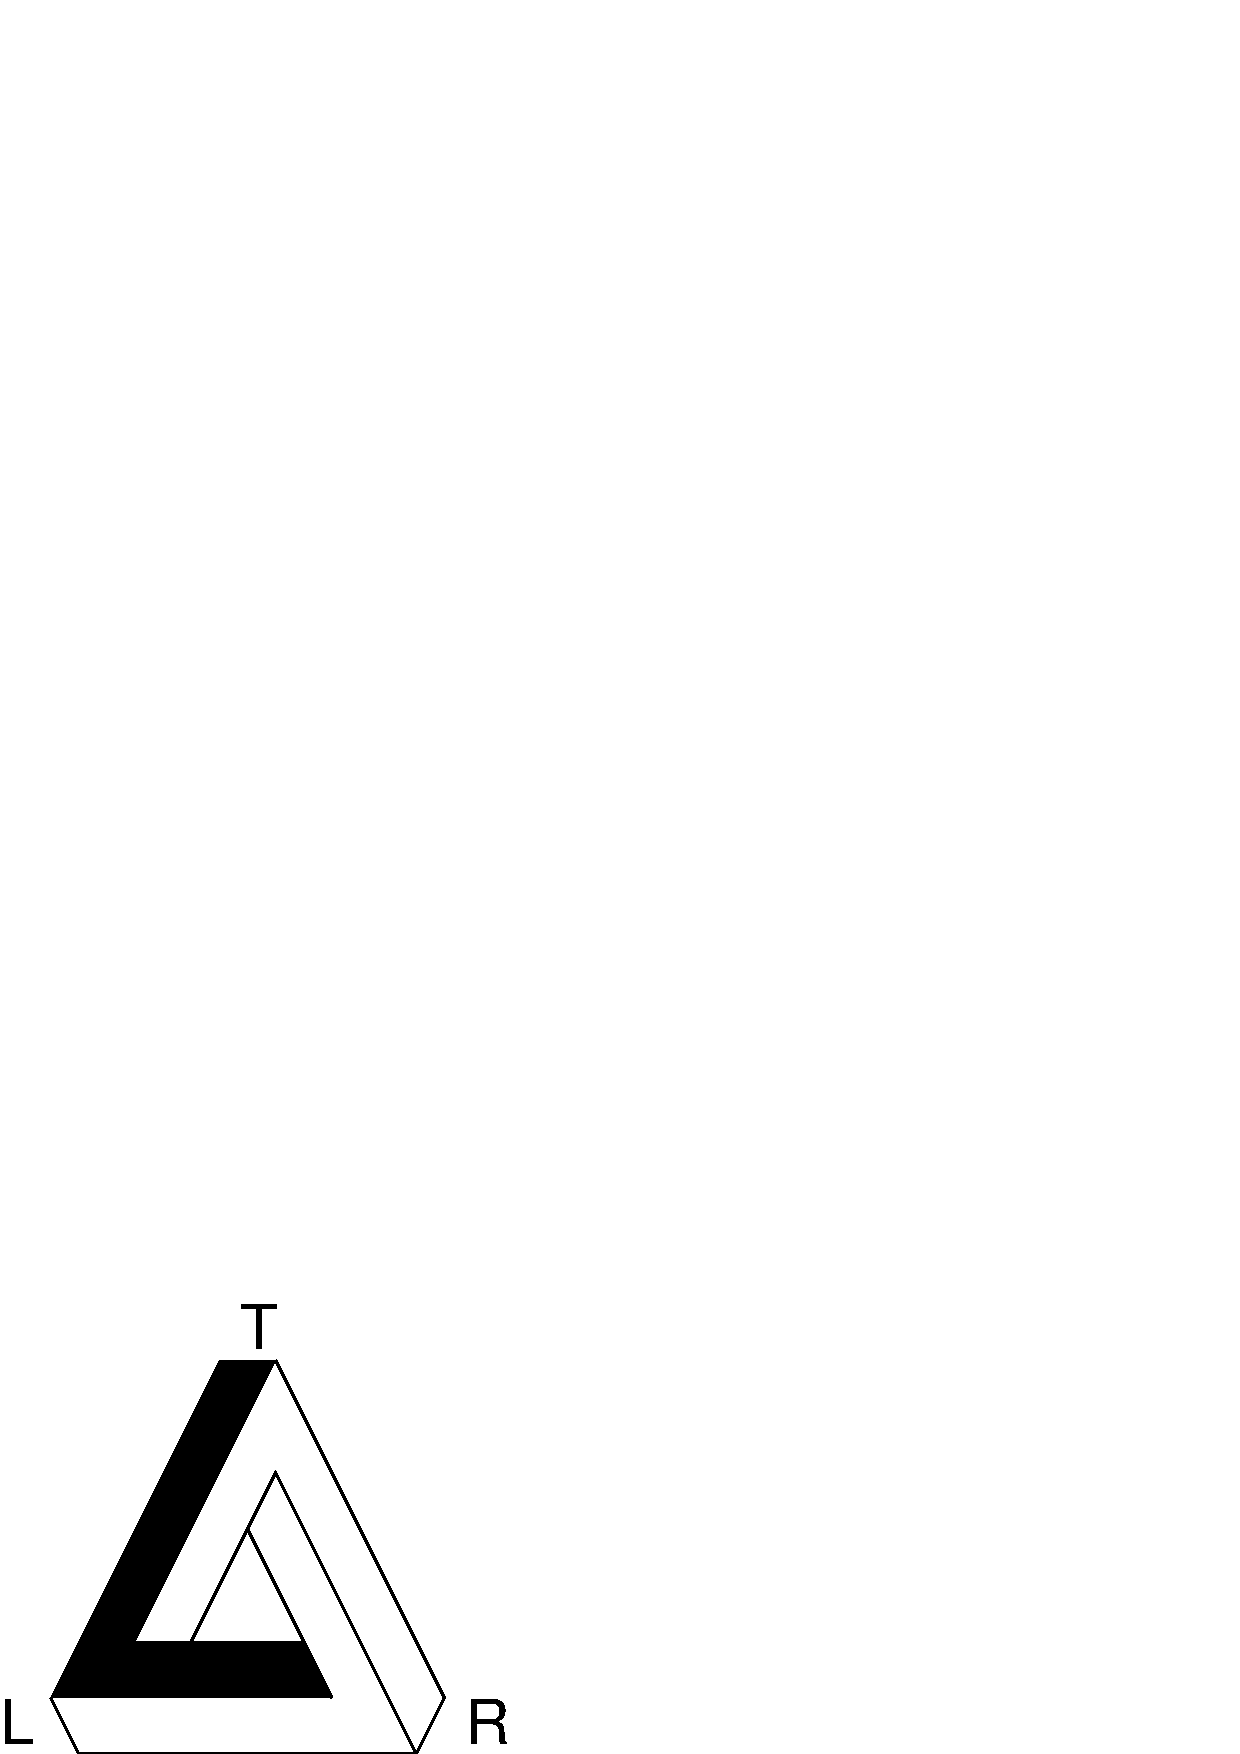
\includegraphics{escher}}
 \source{Guy Shaw}
 \caption{An illustration taken
          from~\cite{A-W:MG04}}
 \label{fig:a}
\end{figure}
\end{verbatim}
resulting in figure \vref{fig:a}.
\begin{figure}[!b]
 \resizebox{.7\columnwidth}{!}
  {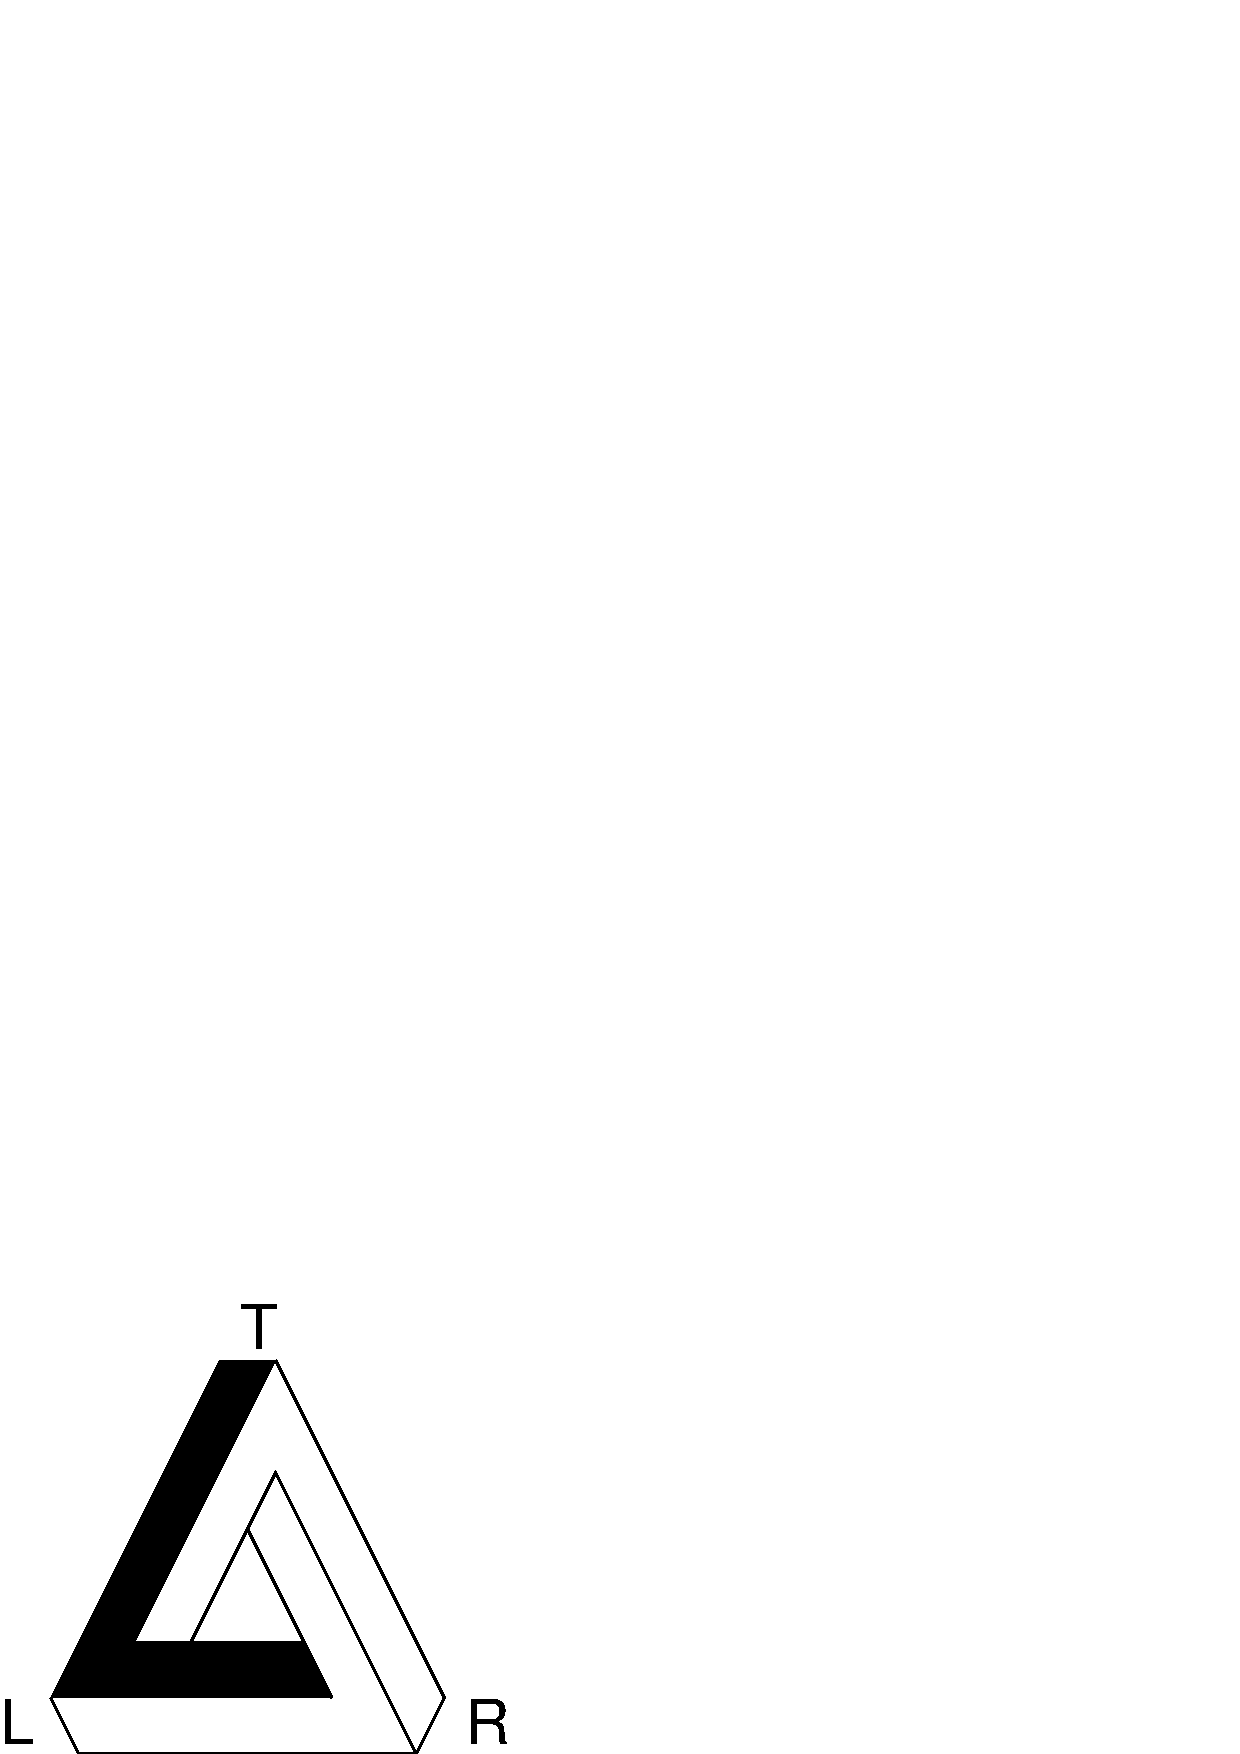
\includegraphics[draft=false]{escher}}
 \source{Guy Shaw}
 \caption{An illustration taken
          from~\cite{A-W:MG04}}
 \label{fig:a}
\end{figure}

\subsection{Floats}

Floats are objects which do not have to stay in sync with the running
text but are allowed to move from their original place to some other
position where they fit better for page breaking reasons. Such objects
they are typically numbered so that they can be referenced from within
the running text.

\LaTeX{} by default supports two float types: figures and
tables. These float types are also supported by the \aipcls{} although
their internal implementation is quite different resulting in a number
of important differences in behavior:\footnote{There exist packages
that extend the number of float types. (This information is given as a
footnote to show that footnotes in this class come out below a bottom
float.)}
\begin{itemize}
\item The position of the float caption is determined automatically,
  independently of the placement of the |\caption| command within the
  float body.
\item
  Depending on its width the float automatically spans two
  columns.
  In case of a table the whole object (including its caption)
  might be rotated automatically if its exceeds |\textwidth|.
\item The body of the float environments are processed in L-R mode and
  not in paragraph mode as in standard \LaTeX. This is necessary for
  measuring its width. Thus if paragraph mode is needed one has to put
  a \texttt{minipage} environment of the appropriate width (e.g.,
  |\columnwidth|) into the body.
\item Only one |\caption| command per float is allowed.
\end{itemize}

\subsubsection{Figures}


\BDefE{figure}[o]{pos}

Like with standard \LaTeX{} the optional \Larg{pos} argument can be
used to specify into which float areas this float is allowed to
migrate (default is |tbp|).

The environment \texttt{figure*} is not supported as figures that need
to span both columns are automatically recognized in two column mode.

\BDefC{source}[m]{text}
Command to specify the origin of the picture shown. The \Larg{text}
will be printed in small italics below the illustration.

A typical example of a figure float would be
\begin{verbatim}
\begin{figure}
 \resizebox{.8\textwidth}{!}
           {
\includegraphics{outline}}
 \caption{PostScript example taken
          from~\cite{A-W:MG04}}
 \label{fig:b}
 \source{F. Mittelbach}
\end{figure}
\end{verbatim}
The result is shown in Figure~\vref{fig:b}.

\begin{figure}
\resizebox{.8\textwidth}{!}{
\includegraphics[draft=false]{outline}}
\caption{PostScript example taken from~\cite{A-W:MG04}}
\label{fig:b}
\source{F. Mittelbach}
\end{figure}

\BDefC{spaceforfigure}[mm]{horizontal}{vertical}
If the illustration is to be manually pasted into the final document
one can leave the right amount of space by using this command as
follows:
\begin{verbatim}
\begin{figure}
 \spaceforfigure{2in}{1cm}
 \caption{Caption for a figure to be
          pasted in later}
 \label{fig:3}
 \source{F. Mittelbach}
\end{figure}
\end{verbatim}
All standard \TeX{} units can be used to specify the space needed. The
above example make room for an illustration that is two inches wide and
one centimeter high. The result is shown as Figure~\vref{fig:3}.

\begin{figure}
 \spaceforfigure{2in}{1cm}
 \caption{Caption for a figure to be
          pasted in later}
 \label{fig:3}
 \source{F. Mittelbach}
\end{figure}

\subsubsection{Tables}

\BDefE{table}[o]{pos}

Like with standard \LaTeX{} the optional \Larg{pos} argument can be
used to specify into which float areas this float is allowed to
migrate (default is |tbp|).

The environment \texttt{table*} is not supported as tables that need
to span both columns are automatically recognized in two column mode.

Typically the body of the environment would consist of a
\texttt{tabular} environment responsible for producing the actual
table including the table and stub headers.

\BDefC{tablehead}[mmmm]{cols}{h-pos}{v-pos}{heading text}

To ease the production of tables the command |\tablehead| is provided
which is essentially and abbreviation for a |\multicolumn| command
that additionally boldens its text argument. I.e., \Larg{cols}
specifies the number of columns the \Larg{heading text} should span
and \Larg{h-pos} defines the horizontal positioning of the text of the
column(s), e.g., |l|, |r|, |c|, or |p{...}|.  In contrast to a simple
|\multicolumn| command the \Larg{heading text} can be split vertically
by using |\\| to denote the line breaks.  The \Larg{v-pos} argument
should contain either |t|, |c|, or |b| denoting the vertical placement
of the text in relation to other cells of that row. It is only
relevant if the \Larg{heading text} consists of more than one
line. See the example table \vpageref[below]{tab:source} that
demonstrates the use of this command.

\BDefC{source}[m]{text} Command to specify the origin of the data
given in the table. The \Larg{text} will be printed in small italics
below the table.

\BDefC{tablenote}[m]{text}

Command to produce a note to the table. It can only be used within a
\texttt{table} environment and should be used only at the right
end of a table cell. The command produces a raised footnote symbol at
the place used which sticks into the right margin. As far as \LaTeX{}
is concerned this symbol does not occupy any space. Thus is will not
modify the alignment of table columns. The \Larg{text} will appear
below the table.

In the current release notes to |\caption| or |\source| are not
possible.

\BDefC{tablenote*}[m]{text}
Like |\tablenote| but this time the raised footnote symbol will occupy
space. This version is intended to be used in the middle of cells.

An example showing the use of all commands described above is shown in
Table~\vref{tab:a}. It was produced by the following input:\label{tab:source}
\begin{verbatim}
\begin{table}
\begin{tabular}{lrrrr}
\hline
 &\tablehead{1}{r}{b}{Single\\outlet}
 &\tablehead{1}{r}{b}{Small\tablenote
       {2-9 retail outlets}\\multiple}
 &\tablehead{1}{r}{b}{Large\\multiple}
 &\tablehead{1}{r}{b}{Total}   \\
\hline
1982 & 98  & 129 & 620    & 847\\
1987 & 138 & 176 & 1000  & 1314\\
1991 & 173 & 248 & 1230  & 1651\\
1998\tablenote{predicted}
     & 200 & 300 & 1500  & 2000\\
\hline
\end{tabular}
\source{Central Statistical Office,
        UK}
\caption{Average turnover per shop: by
  type of retail organisation}
\label{tab:a}
\end{table}
\end{verbatim}

\begin{table}
\begin{tabular}{lrrrr}
\hline
  & \tablehead{1}{r}{b}{Single\\outlet}
  & \tablehead{1}{r}{b}{Small\tablenote{2-9 retail outlets}\\multiple}
  & \tablehead{1}{r}{b}{Large\\multiple}
  & \tablehead{1}{r}{b}{Total}   \\
\hline
1982 & 98 & 129 & 620    & 847\\
1987 & 138 & 176 & 1000  & 1314\\
1991 & 173 & 248 & 1230  & 1651\\
1998\tablenote{predicted} & 200 & 300 & 1500  & 2000\\
\hline
\end{tabular}
\source{Central Statistical Office, UK}
\caption{Average turnover per shop: by type
  of retail organisation}
\label{tab:a}
\end{table}

\BDefC{setlength}[mm]{\texttt{\upshape\string\hlinesep}}{value}

Vertical spacing between horizontal lines produced from |\hline|
inside a tabular environment is controlled by the length parameter
|\hlinesep| in this class. The default value (1pt) gives one point
extra space above such lines and three times as much (i.e. 3pt) extra
space below. This is done to implement the layout requirements for
tables in the AIP proceedings (which are not supposed to have vertical
lines in the tables). If tables with vertical lines are necessary for
some reason, then the value of this parameter should be set to
\texttt{0pt} either globally for the whole document or locally within
the \texttt{table} environment. Otherwise the vertical lines will have
strange gaps whenever a |\hline| command is used to produce a
horizontal line.

\subsubsection{Counters}

The |\alph| and |\fnsymbol| commands to represent counter values have
extended ranges. For example |\alph| will now count up to 52 (zz) and
the |\fnsymbol| command will produce the following symbols
\makeatletter
\@fnsymbol{1},
\@fnsymbol{2},
\@fnsymbol{3},
\@fnsymbol{4},
\@fnsymbol{5},
\@fnsymbol{6},
\@fnsymbol{7},
\@fnsymbol{8},
\@fnsymbol{9},
\@fnsymbol{10},
\@fnsymbol{11},
\@fnsymbol{12},
\@fnsymbol{13},
\@fnsymbol{14},
\@fnsymbol{15}, and
\@fnsymbol{16}.
\makeatother
This will allow for up to 16 table notes per table. For documents that
need a larger number of table notes select the option
\texttt{tnotealph} to switch to lower case alphabetic letters to mark
such notes.

\subsubsection{Long tables}

Tables which are longer than one page cannot be placed into a
\texttt{table} environment as floats cannot have a size larger than a
page. Such tables are supported by the standard \LaTeX{} package
\texttt{longtable} written by David Carlisle. However this package
only works in single column mode.

With two-column layouts, such as the one for the AIP 8x11 double
column proceedings, such tables can only be added at the end of the
paper by preceding the |longtable| environments with a |\onecolumn|
declaration.

The package is supported by the class in the sense that captions
within a \texttt{longtable} environment will be formatted using the
appropriate style; however in contrast to the \texttt{table}
environment it is the responsibility of the user to place the caption
at the top of the table. The commands |\source| and |\tablenote| are
not supported within this environment, but the |\tablehead| command
can be used to produce column heads if desired.

Refer to the \texttt{longtable} package documentation or to
\cite[p.122ff]{A-W:LLa94} for a detailed description of the syntax of
the \texttt{longtable} environment.

A possible alternative is the package \texttt{supertabular} written by
Johannes Braams; however in this case no attempt has been made to
ensure that a table produced with \texttt{supertabular} conforms to
the layout specification for the \aipcls{}. Be aware that this package
defines its own |\tablehead| command (with a completely different
function).

Refer to the package documentation for the syntax description. A
detailed comparison between \texttt{supertabular} and
\texttt{longtable} can be found in Chapter~5 of \cite{A-W:LLa94}.

\subsubsection{Building floats manually}

The original \LaTeX{} environments \texttt{figure} and \texttt{table}
as well as their star forms are still available under the names
\texttt{ltxfigure} and \texttt{ltxtable}. They should not be used in
normal circumstances but are provided in case the automatism of
the \aipcls{} needs overwriting.

Please note that if these environments are used the position of the
|\caption| command determines the placement of the caption within the
float body and that the special commands for figures and tables, e.g.,
|\tablenote|, etc.\ as provided by this class are not available within
these environments.

\begin{table}[!t]
%%
%% Next lines change table font size if the layoutstyle name doesn't
%% start with 8 (ie is not 8x11single or 8x11double)
\makeatletter
\if8\expandafter\@car\selectedlayoutstyle\@nil\relax
\else
  \fontsize{7}{8}\selectfont
\fi
\makeatother
%%
%% End hack
%%
\begin{tabular}{rrrp{.6\textwidth}} % .4\textwidth
\hline
  \tablehead{1}{r}{b}{File} &
  \tablehead{1}{c}{b}{Date} &
  \tablehead{1}{c}{b}{Version} &
  \tablehead{1}{c}{b}{Description} \\
\hline
 aipproc.cls &    2000/08/31 & v1.2a & AIP Proceedings (FMi) \\
fixltx2e.sty &    1999/12/01 & v1.0b & fixes to LaTeX \\
    calc.sty &    1998/07/07 & v4.1b & Infix arithmetic (KKT,FJ) \\
  ifthen.sty &    1999/09/10 & v1.1b & Standard LaTeX ifthen package (DPC) \\
graphicx.sty &    1999/02/16 & v1.0f & Enhanced LaTeX Graphics (DPC,SPQR) \\
  keyval.sty &    1999/03/16 & v1.13 & key=value parser (DPC) \\
graphics.sty &    1999/02/16 & v1.0l & Standard LaTeX Graphics (DPC,SPQR) \\
    trig.sty &    1999/03/16 & v1.09 & sin cos tan (DPC) \\
graphics.cfg & \\
   dvips.def &    1999/02/16 & v3.0i & Driver-dependant file (DPC,SPQR) \\
     url.sty &    1999/03/28 &  ver 1.5x  & Verb mode for urls, etc. \\
 article.cls &    2000/05/19 & v1.4b & Standard LaTeX document class \\
  size10.clo &    2000/05/19 & v1.4b & Standard LaTeX file (size option) \\
  aipxfm.sty & \\
 mathptm.sty &   2000/01/12 &PSNFSS-v8.1 &Times + math package (SPQR) \\
   times.sty &   2000/01/12 &PSNFSS-v8.1 &Times font as default roman(SPQR) \\
  ot1ptm.fd  &  2000/01/12  &PSNFSS-v8.1 & font definitions for OT1/ptm. \\
 fontenc.sty & \\
   t1enc.def &   2000/08/30 & v1.91 &Standard LaTeX file \\
   t1ptm.fd  &  2000/01/12  &PSNFSS-v8.1 & font definitions for T1/ptm. \\
textcomp.sty &   2000/08/30 &v1.91 &Standard LaTeX package \\
  ts1enc.def &   1998/06/12 & v3.0d & (jk/car/fm) Standard LaTeX file \\
varioref.sty &   1999/12/02 &v1.2c &package for extended references (FMi) \\
  aip-8s.clo & \\
ttct0001.sty & \\
shortvrb.sty &   2000/07/04  &v2.0m & Standard LaTeX documentation package
 (FMi) \\
hyperref.sty &   2000/05/08  &v6.70f & Hypertext links for LaTeX \\
  pd1enc.def &   2000/05/08  &v6.70f & Hyperref: PDFDocEncoding definition
 (HO) \\
hyperref.cfg & \\
  hdvips.def &   2000/05/08  &v6.70f & Hyperref driver for dvips \\
 pdfmark.def &   2000/05/08  &v6.70f & Hyperref definitions for pdfmark
 specials \\
  ts1cmr.fd  &  1999/05/25  &v2.5h & Standard LaTeX font definitions \\
 nameref.sty &   2000/05/08  &v2.18 & Cross-referencing by name of section \\
   t1pcr.fd  &  2000/01/12  &PSNFSS-v8.1 & font definitions for T1/pcr. \\
ot1ptmcm.fd  &  2000/01/03  &Fontinst v1.801 & font definitions for
 OT1/ptmcm. \\
omlptmcm.fd  &  2000/01/03  &Fontinst v1.801 & font definitions for
 OML/ptmcm. \\
omspzccm.fd  &  2000/01/03  &Fontinst v1.801 & font definitions for
 OMS/pzccm. \\
omxpsycm.fd  &  2000/01/03 & Fontinst v1.801  &font definitions for
 OMX/psycm. \\
  ts1ptm.fd  &  2000/01/12 & PSNFSS-v8.1  &font definitions for TS1/ptm. \\
  escher.eps &   &&  Graphic file (type eps) \\
 outline.eps &  & &  Graphic file (type eps)  \\
\hline
\end{tabular}
\caption{Files used by the \aipcls{}}
\label{tab:b}
\source{Output of \texttt{\string\listfiles} when processing
        \texttt{aipguide.tex}}

\end{table}


\subsection{Urls}

\BDefC{url}[m]{data}

For documenting URLs and related data the |\url| command is provided.
It allows breaking the URL in certain places and typesets it in an
adequate font and format. Instead of using curly brackets the argument
can be delimited by two identical characters not used in the argument.

\subsection{Bibliography}

Referring to other articles, books, etc.\ can be done using the |\cite|
command of standard \LaTeX{}. The list of references itself can
either be produced using standard \LaTeX{} methods or using
\textsc{Bib}\TeX.

If installed, the \aipcls{} class includes the \texttt{natbib} system
which offers an extended set of citation commands. These commands have
been originally developed to support author/year citation styles but
are also useful with numerical citation styles.


The \texttt{natbib} system has two basic citation commands, |\citet| and
|\citep| for \emph{textual} and \emph{parenthetical} citations, respectively.
There also exist the starred versions |\citet*| and |\citep*| that print
the full author list, and not just the abbreviated one.
All of these may take one or two optional arguments to add some text before
and after the citation. Table~\vref{tab:natbib} shows some examples.
\begin{table}
\begin{tabular}{@{}l@{\quad$\Rightarrow$\quad}l}
\hline
\multicolumn{2}{@{}l}{\bfseries Author/year style} \\
\hline
  |\citet{jon90}| & Jones et al. (1990)\\
  |\citet[chap.~2]{jon90}| & Jones et al. (1990, chap.~2)\\[0.5ex]
  |\citep{jon90}| & (Jones et al., 1990)\\
  |\citep[chap.~2]{jon90}| & (Jones et al., 1990, chap.~2)\\
  |\citep[see][]{jon90}| & (see Jones et al., 1990)\\
  |\citep[see][chap.~2]{jon90}| & (see Jones et al., 1990, chap.~2)\\[0.5ex]
  |\citet*{jon90}| & Jones, Baker, and Williams (1990)\\
  |\citep*{jon90}| & (Jones, Baker, and Williams, 1990) \\
\hline
\multicolumn{2}{@{}l}{\bfseries Numerical style} \\
\hline
  |\citet{jon90}| & Jones et al. [21]\\
  |\citet[chap.~2]{jon90}| & Jones et al. [21, chap.~2]\\[0.5ex]
  |\citep{jon90}| & [21]\\
  |\citep[chap.~2]{jon90}| & [21, chap.~2]\\
  |\citep[see][]{jon90}| & [see 21]\\
  |\citep[see][chap.~2]{jon90}| & [see 21, chap.~2]\\[0.5ex]
  |\citep{jon90a,jon90b}| & [21, 32]\\
\hline
\end{tabular}
\caption{Example of \texttt{natbib} commands and their results}
\label{tab:natbib}
\end{table}
There are many more commands and variants, see \cite{man:Daly99a} or
\cite{man:Daly99b} for further details.

\subsubsection{Bibliography produced manually}

\BDefE{thebibliography}[m]{widest-label}

Environment to hold the list of references.

\BDefC{bibitem}[m]{label}

Command to start a bibliographical entry having the label \Larg{label}
for use in |\cite| commands. Refer to the publishers manual, e.g.,
\cite{man:aipproceed}, for information on how to lay out individual
entries. For example:
\begin{verbatim}
\bibitem{Brown2000}
   M.~P. Brown and K. Austin,
  \emph{The New Physique},
  Publisher Name, Publisher City,
  2000, pp. 212--213.
\end{verbatim}

If commands from \texttt{natbib} (e.g., from table~\ref{tab:natbib})
should be usable, then additional information has to be passed to the
|\bibitem| via an optional argument.

\BDefC{bibitem}[om]{display-info}{label}

The optional argument \Larg{display-info} should then, and only then,
contain the author(s) name(s) followed by the year in parentheses
without any spaces, for example:
\begin{verbatim}
\bibitem[Brown and Austin(2000)]
        {Brown2000}
  ...
\end{verbatim}
The essential feature is that the label (the part in brackets) consists
of the author names, as they should appear in the citation, with the year
in parentheses following. There must be no space before the opening
parenthesis!
This will be automatically produced if \BibTeX{} is used.

\subsubsection{Bibliography produced using \textsc{Bib}\TeX}

The \aipcls{} is accompanied by \BibTeX{} style files which can be used
to produce compliant reference lists from \BibTeX{} database
files. To use \BibTeX{} one first has to run the source file through
\LaTeX{} then run \BibTeX{} and then rerun \LaTeX{} twice to get all
references resolved. \BibTeX{} is described in more detail in appendix
B of \cite{A-W:LLa94} and in chapter~13 of \cite{A-W:MG04}.

\BDefC{bibliographystyle}[m]{style-name}
This declaration specifies to \BibTeX{} that the style
\Larg{style-name} should be used. It can be placed anywhere within the
document but is usually positioned directly in front of the command
described below.

For a discussion which of the supplied \BibTeX{} styles should be used
for which proceedings see the section ``Special requirements\ldots''
below.

\BDefC{bibliography}[m]{bib-list}

This command denotes the position where the reference list produced by
\BibTeX{} will be included in the document. The \Larg{bib-list} is a
comma separated list of \BibTeX{} database files.

\section{General requirements and restrictions}

This class was designed to work with \LaTeXe{} release 1999/06/01 or a
later version. Earlier releases may work but have not been tested.

With the exception of the packages \texttt{natbib} and \texttt{url} it
only requires files which are part of a standard \LaTeX{}
distribution, i.e., it should work if your installation contains the
following components:
\texttt{base}, \texttt{tools}, \texttt{graphics}, and \texttt{psnfss},
see \vref{tab:b} for files used to produce this document.

The most recent \LaTeX{} distribution as well as \texttt{natbib} and
\texttt{url} can be obtained from CTAN sites (Comprehensive \TeX{}
Archive Network).

Refer to \url{http://www.tug.org} for more information on CTAN and
\TeX{} in general.

A ready to run \TeX{} system for various platforms which has
everything required is available on CD-ROM, look into
\url{http://www.tug.org/texlive.html}.

This \TeX{} implementation is also made available as an add-on to
several books on \LaTeX, e.g., \cite{A-W:KD04,A-W:MG04}.

For loading individual packages from a CTAN archive refer to
\url{http://www.ctan.org} and search for the package name. Please omit
extensions such as \texttt{.sty} when searching, e.g., search for
\texttt{natbib} rather than \texttt{natbib.sty}, as such packages are
often distributed in source form only, e.g., as a \texttt{.dtx} file.

It is also possible to download a complete \TeX/\LaTeX{} installation
from CTAN, e.g., Miktex + Winedit + Ghostview. Finally, it is also
possible to download a CD-ROM image of the \TeX-live CD from CTAN
(roughly 300MB): search for \texttt{texlive} (and make sure you select
a suitable mirror near you).

\section{Special requirements for individual layouts}

\subsection{AIP proceeding layout 6x9}

\begin{itemize}
\raggedright
\item
 The entire paper will be reduced 15\% in the printing process. Please
 make sure all figures as well as the text within the figures are
 large enough in the manuscript to be readable in the finished book.
\item
 The use of the |\source| command is discouraged.
\item
 Compliant \BibTeX{} styles are \texttt{aipproc} (for use with
 \texttt{natbib}) and  \texttt{aipprocl} (if \texttt{natbib} is
 missing at the site).
\item
 The options \texttt{bibliocites} and \texttt{numberedheadings} have
 no effect.
\end{itemize}

\subsection{AIP proceeding layout 8x11 single/double}

\begin{itemize}
\raggedright
\item
 The use of the |\source| command is discouraged.
\item
 Compliant \BibTeX{} styles are \texttt{aipproc} (for use with
 \texttt{natbib}) and  \texttt{aipprocl} (if \texttt{natbib} is
 missing at the site).
\item
 The options \texttt{bibliocites} and \texttt{numberedheadings} have
 no effect.
\end{itemize}

\subsection{ARLO}

Note: the ARLO layout is no longer supported.

\begin{itemize}
\raggedright
\item
A copyright year (|\copyrightyear|) needs to be provided.

\item
Pacs numbers should be provided (|\classification|).

\item
  The \texttt{arlo} layout offers one additional environment to specify
  multimedia files:
\begin{verbatim}
\begin{multimedia}
 \multimediauid{523}
 \multimediatype{gif}
 \multimediasize{1.2Mb}
 \multimediaurl{http://yorktown.%
       eng.yale.edu/test/msXXX/}
 \multimediacaption{Fancy video}
 \label{fv} % label is optional
\end{multimedia}
\end{verbatim}
  References to a multimedia file can be made using |\label| and
  |\ref|. Instead of the latter command |\multimediaref| can be used
to automatically get the appropriate frills, e.g., `Mm.~2' instead of
just `2' as produced by |\ref|.

\item
  Select the \texttt{draft} option for the initial submission and the
  copy-editing stage. Replace it by the \texttt{final} option when
  producing the final paper, so that page numbers and other
  items are stripped away.

\item
  To conform to the layout specification for citations the
  \texttt{natbib} system has to be installed.

\item
 For ARLO two compliant \BibTeX{} styles are available:
 \texttt{arlonum} should be used together with the class option
 \texttt{numcites}, while \texttt{arlobib} should be used together with
 the option \texttt{bibliocites}.

\item
 The options \texttt{bibliocites} and \texttt{numberedheadings} can be
 used to switch to author/year citation scheme and numbered headings,
 respectively.
\end{itemize}


\begin{thebibliography}{1}

\bibitem{man:aipproceed}
American Institute of Physics, \emph{Conference Proceedings: Instructions for
  Camera Ready Manuscripts}, Feb 2000.

\bibitem{man:Daly99a}
P. Daly, \emph{Natural Sciences Citations and References
  (Author--Year and Numerical Schemes)},
  1999, distributed as \texttt{natbib.dtx} with the \texttt{natbib} software.

\bibitem{man:Daly99b}
P. Daly, \emph{Reference sheet for \texttt{natbib} usage},
  1999, distributed as \texttt{natnotes.tex} with the  \texttt{natbib}
  software.

\bibitem{A-W:KD04}
H.~Kopka and P.~Daly, \emph{Guide to {\LaTeX}}, Tools and
  Techniques for Computer Typesetting, Addison-Wesley, Boston, Massachusetts,
  2004, 4 edn., ISBN 0-321-17385-6.

\bibitem{A-W:MG04}
F.~Mittelbach and M.~Goossens, \emph{The {\LaTeX} Companion}, Tools and
  Techniques for Computer Typesetting, Addison-Wesley, Boston, Massachusetts,
  2004, 2 edn., ISBN 0-201-36299-6, with Johannes Braams, David Carlisle, and
  Chris Rowley.

\bibitem{A-W:GMR97}
M.~Goossens, S.~Rahtz, and F.~Mittelbach, \emph{The {\LaTeX} Graphics
  Companion}, Tools and Techniques for Computer Typesetting, Addison-Wesley,
  Reading, Massachusetts, 1997, ISBN 0-201-85469-4.

\bibitem{A-W:LLa94}
L.~Lamport, \emph{{\LaTeX:} A Document Preparation System}, Addison-Wesley,
  Reading, Massachusetts, 1994, second edn.

\end{thebibliography}
\end{document}
\endinput
%%
%% End of file `aipguide.tex'.
